\begin{figure}[htp]
\centering
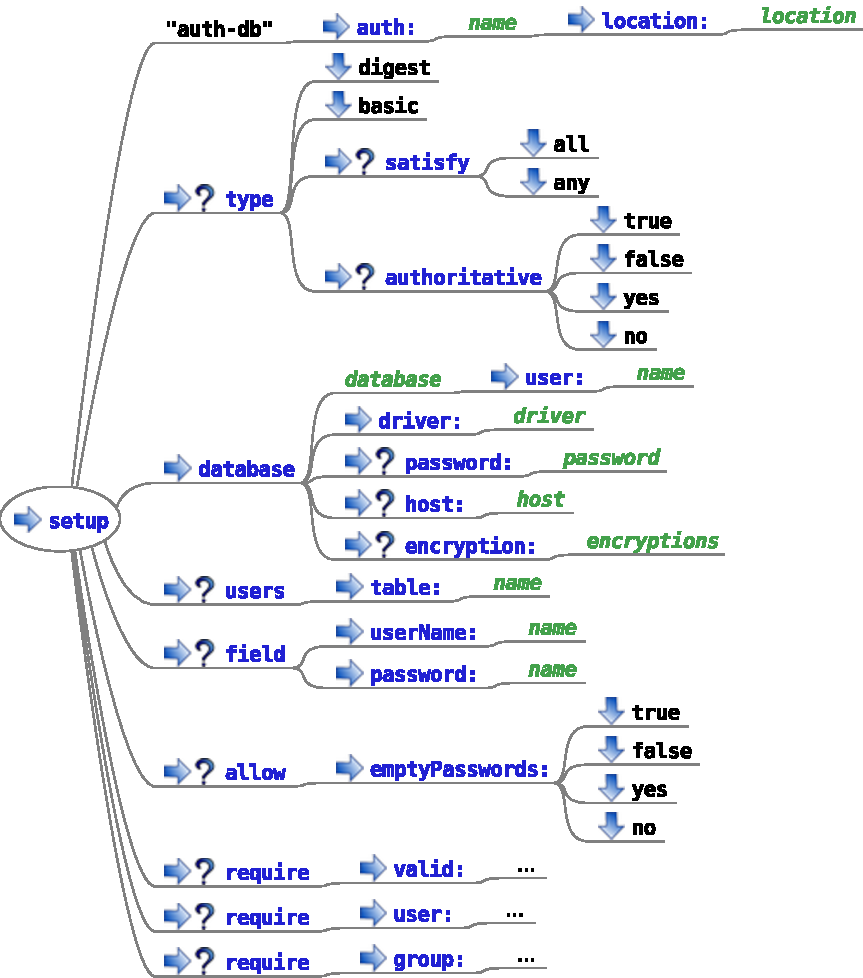
\includegraphics[width=0.8\textwidth]{httpd_setup_auth_db_script}
\label{fig:httpd_setup_auth_db_script}
\caption{Httpd Database Authentication Statements}
\end{figure}

%% setup auth-db
\TheStatement[httpd:domain:setup-auth-db]{setup ``auth-db''}
\TheStatement*[httpd!domain!setup!auth-db]{setup ``auth-db'', auth: \Arg{name}, location: \Arg{location}, \{ type require \}}

Configures authentication with a relational database as the storage for groups and users,
with the \Arg{name} of the authentication and the \Arg{location} that is 
restricted.

\begin{lstlisting}[style=Java]
httpd {
    domain "test1.com", address: "192.168.0.50", {
        setup "auth-db", auth: "Private Directory", location: "/private", {
        }
    }
}
\end{lstlisting}

%% database
\TheStatement[httpd:domain:setup-auth-db-database]{database}
\TheStatement*[httpd!domain!setup!auth-db!database]{database \Arg{database}, user: \Arg{name}, password: \Arg{password}, driver: \Arg{driver} [, host: \Arg{host}] [, encryption: \Arg{encryptions}]}

Sets the database back-end.

\begin{lstlisting}[style=Java]
httpd {
    domain "test1.com", address: "192.168.0.50", {
        setup "auth-ldap", auth: "Private Directory", location: "/private", {
            database "authdb", user: "userdb", password: "userpassdb", host: "localhost", driver: "mysql"
        }
    }
}
\end{lstlisting}

